

\documentclass{article}
\usepackage[utf8]{inputenc}
\usepackage[a4paper, total={6in, 10in}]{geometry}
\usepackage{braket}
\usepackage{xcolor}
\usepackage{amsmath}
\usepackage{amsfonts}
\usepackage{graphicx}
\usepackage{float}
% \usepackage{biblatex} %Imports biblatex package

\usepackage[
backend=biber,
style=alphabetic,
sorting=ynt
]{biblatex}

\begin{document}

\newcommand{\GG}{\tilde{G} }
\newcommand{\TGG}{\(\tilde{G}\) }
\newcommand{\Prb}[1]{ \mathbf{Pr}\left[ {#1} \right] }
\newcommand{\commentt}[1]{\textcolor{blue}{ \textbf{[COMMENT]} #1}}
\newcommand{\ctt}[1]{\commentt{#1}}
\newcommand{\prb}[1]{ \mathbf{Pr} \left[ {#1} \right]}
\newcommand{\onotation}[1]{\(\mathcal{O} \left( {#1}  \right) \)}
\newcommand{\ona}[1]{\onotation{#1}}
\newcommand{\norm}[1]{\left\lVert#1\right\rVert}
\newcommand{\Ov}[2]{\overset{\text{#1}}{\overbrace{#2}}}
\graphicspath{ {./images/} }


% --------- commands for protocols --------------%

\newcommand{\PP}{\mathcal{P} }
\newcommand{\Ue}{ U_{\delta,\varepsilon } }
% -------------- -------------- -----------------%


\title{  Can AVSS all most surly terminate?   }
\author{David Ponarovsky}
\maketitle

\section{Setting.}
We examine quantum protocols for AVSS in an asynchronous environment under Byzantine attack.  Asynchronous means that the adverser chooses when each message gets to its destination. Byzantine attack defines faulty parties as parties that could do any computation, restricted only to information constraints. And by being quantum, the parties and the dealer could exchange qubits (states) and perform and compute any quantum circuit.         

As classic randomization can be achieved by doing measurements, we will allow ourselves to assume that the protocols perform only unitary operations and measurements and still be relevant to randomized protocols.

Verifiable Secret Sharing is a double stages protocol. In the first stage, the dealer sends his secret to every party; then, the parties should vote if the dealer is honest in the second stage.  

\paragraph{Theorem \cite{FLP85}.} Any protocol \(\mathcal{P}\) solving consensus in the asynchronous model that is resilient to even just one crash failure must have an infinite execution. 

\ctt{Todo: cite the paper of Ittai Abraham, Danny Dolev, Gilad Stern [2020], and explain their results.}

Those results raise the following question:  whether the above lower bond is still held for quantum protocols?  In other words, is there a quantum protocol that is both tolerances for faults and all most surely terminates? Another interesting question, can indistinguishability boosting be done even if the parties act quantumly? 


\paragraph{Theorem 1.} Suppose that \( \mathcal{P} \) is an \textbf{AVSS} protocol that tolerates \(f = 1\) Byzantine faults and \textbf{all most surly} terminates. Then for every \( \Gamma \in \left(0, 1\right)\) at least one of the following options is possible.
\begin{enumerate}
    \item A faulty dealer \(D\) has attack in which he wins with probability at least \( \Gamma \).
    \item A faulty party \(B\) has attack in which he wins with probability at least \( 1 - \Gamma \).
\end{enumerate}

\section{Strategy.}

\paragraph{Lemma I.} Let \(\mathcal{P}\) be a protocol (which could use a random and quantum bits) that terminates all most surely. Then for every pair \( \delta,\varepsilon >0 \) there exists a quantum circuit \(U_{\delta,\varepsilon}\) which with at least \(1 - \delta\) probability it \(\varepsilon\)-approximates the protocol. When we think over secrets which shared by \(D\) as an input state \( \ket{\psi_{D}} \) for \(U_{\delta,\varepsilon}\). the That it:  
\begin{equation}
    \prb{\norm{ U_{\delta,\varepsilon}\ket{\psi_{D}} - \mathcal{P}\left(\ket{\psi_{D}}\right)} < \varepsilon} > 1 - \delta      
\end{equation} From now on, we will think over the protocol as a finite depth quantum circuit, which measure only in the end. 

\paragraph{Definition.} 

\paragraph{Lemma II.} Denote by \( H_{succ,1} \subset \mathcal{H} \) the subspace such that for every \begin{equation*}
    \forall \ket{\psi} \in \text{Image} \left( \Ue H_{succ,1} \right) \Rightarrow  \braket{\psi|\Ov{n-f} {11...11}\text{ junk}} > \frac{1}{\sqrt{2}}
\end{equation*}  Similarly let \( H_{fail} \) be the space of inputs that \( \Ue \) doesn't get in into agreement over them (the complementary of \( H_{succ} \)). Then for every \( \ket{ \xi} \in H_{fail} \)  there exists \( \ket{\eta} \in H_{succ} \) and single-qubit operation \( P : \mathcal{H}_2 \rightarrow \mathcal{H}_2 \) such that \( P \otimes I \ket{\xi} =\ket{\eta} \).   

\paragraph{Proof of Theorem 1.} Consider \( \Gamma > 0 \) and assume that the first option doesn't hold. i.e for a.s terminate protocol \( \mathcal{P} \), a faulty dealer doesn't have a strategy in which he wins with probability greater then \( \Gamma \). In particular, when the dealer shares some \( \ket{ \xi} \in H_{fail} \).

Fix \(\varepsilon, \delta > 0\) such that with probability at least \(1-\delta\) the gate \( \Ue \) approximates \( \PP \). Hence we get that  \begin{equation*}
    \braket{ \xi | \Ue | \mathbf{GHZ}} > \frac{1}{\sqrt{2}} 
\end{equation*} 


In particular. let's look at strategy in which the dealer sends for \( n-2 \) parties the secret \( \ket{1} \) and for the remaining party \(B\) he sends the secret \( \ket{0}\). In that case, the corresponded input for the circuit \( U_{\delta, \varepsilon} \) will be
\begin{equation*}
    \ket{\psi_{D}} = \ket{1111...11\Ov{B's share}{0}111..11\Ov{ancillaries}{000...0}}
\end{equation*}


\paragraph{Lemma II.}

We will think over the protocol as a quantum circuit from now on. 
In addition, we will part the circuit into three vertical parts \(R_{A}, R_{B}, R_{C}\) associated with parties \(A, B,\) and \(C\), respectively. Each connection (edge, shared gate) between the parts matches a state exchanging. Visual demonstration can be find in \textbf{Figure 1}.   



\paragraph{Definition.} We will say that a pure state is an \textbf{uncommitted ket} if it matches a case that the non-faulty parties points different values for the secret.  

\paragraph{Lemma II.} Consider a gate \(U\) which act on \(n\) qubits and commute with permutations (symmetrically to the inputs pins). If adverser enters \(\Theta\left(n\right)\) of the input, then he can ensures that the circuit will outputs will have a constant weight over \textbf{uncommitted ket}.  


\begin{figure}[H]
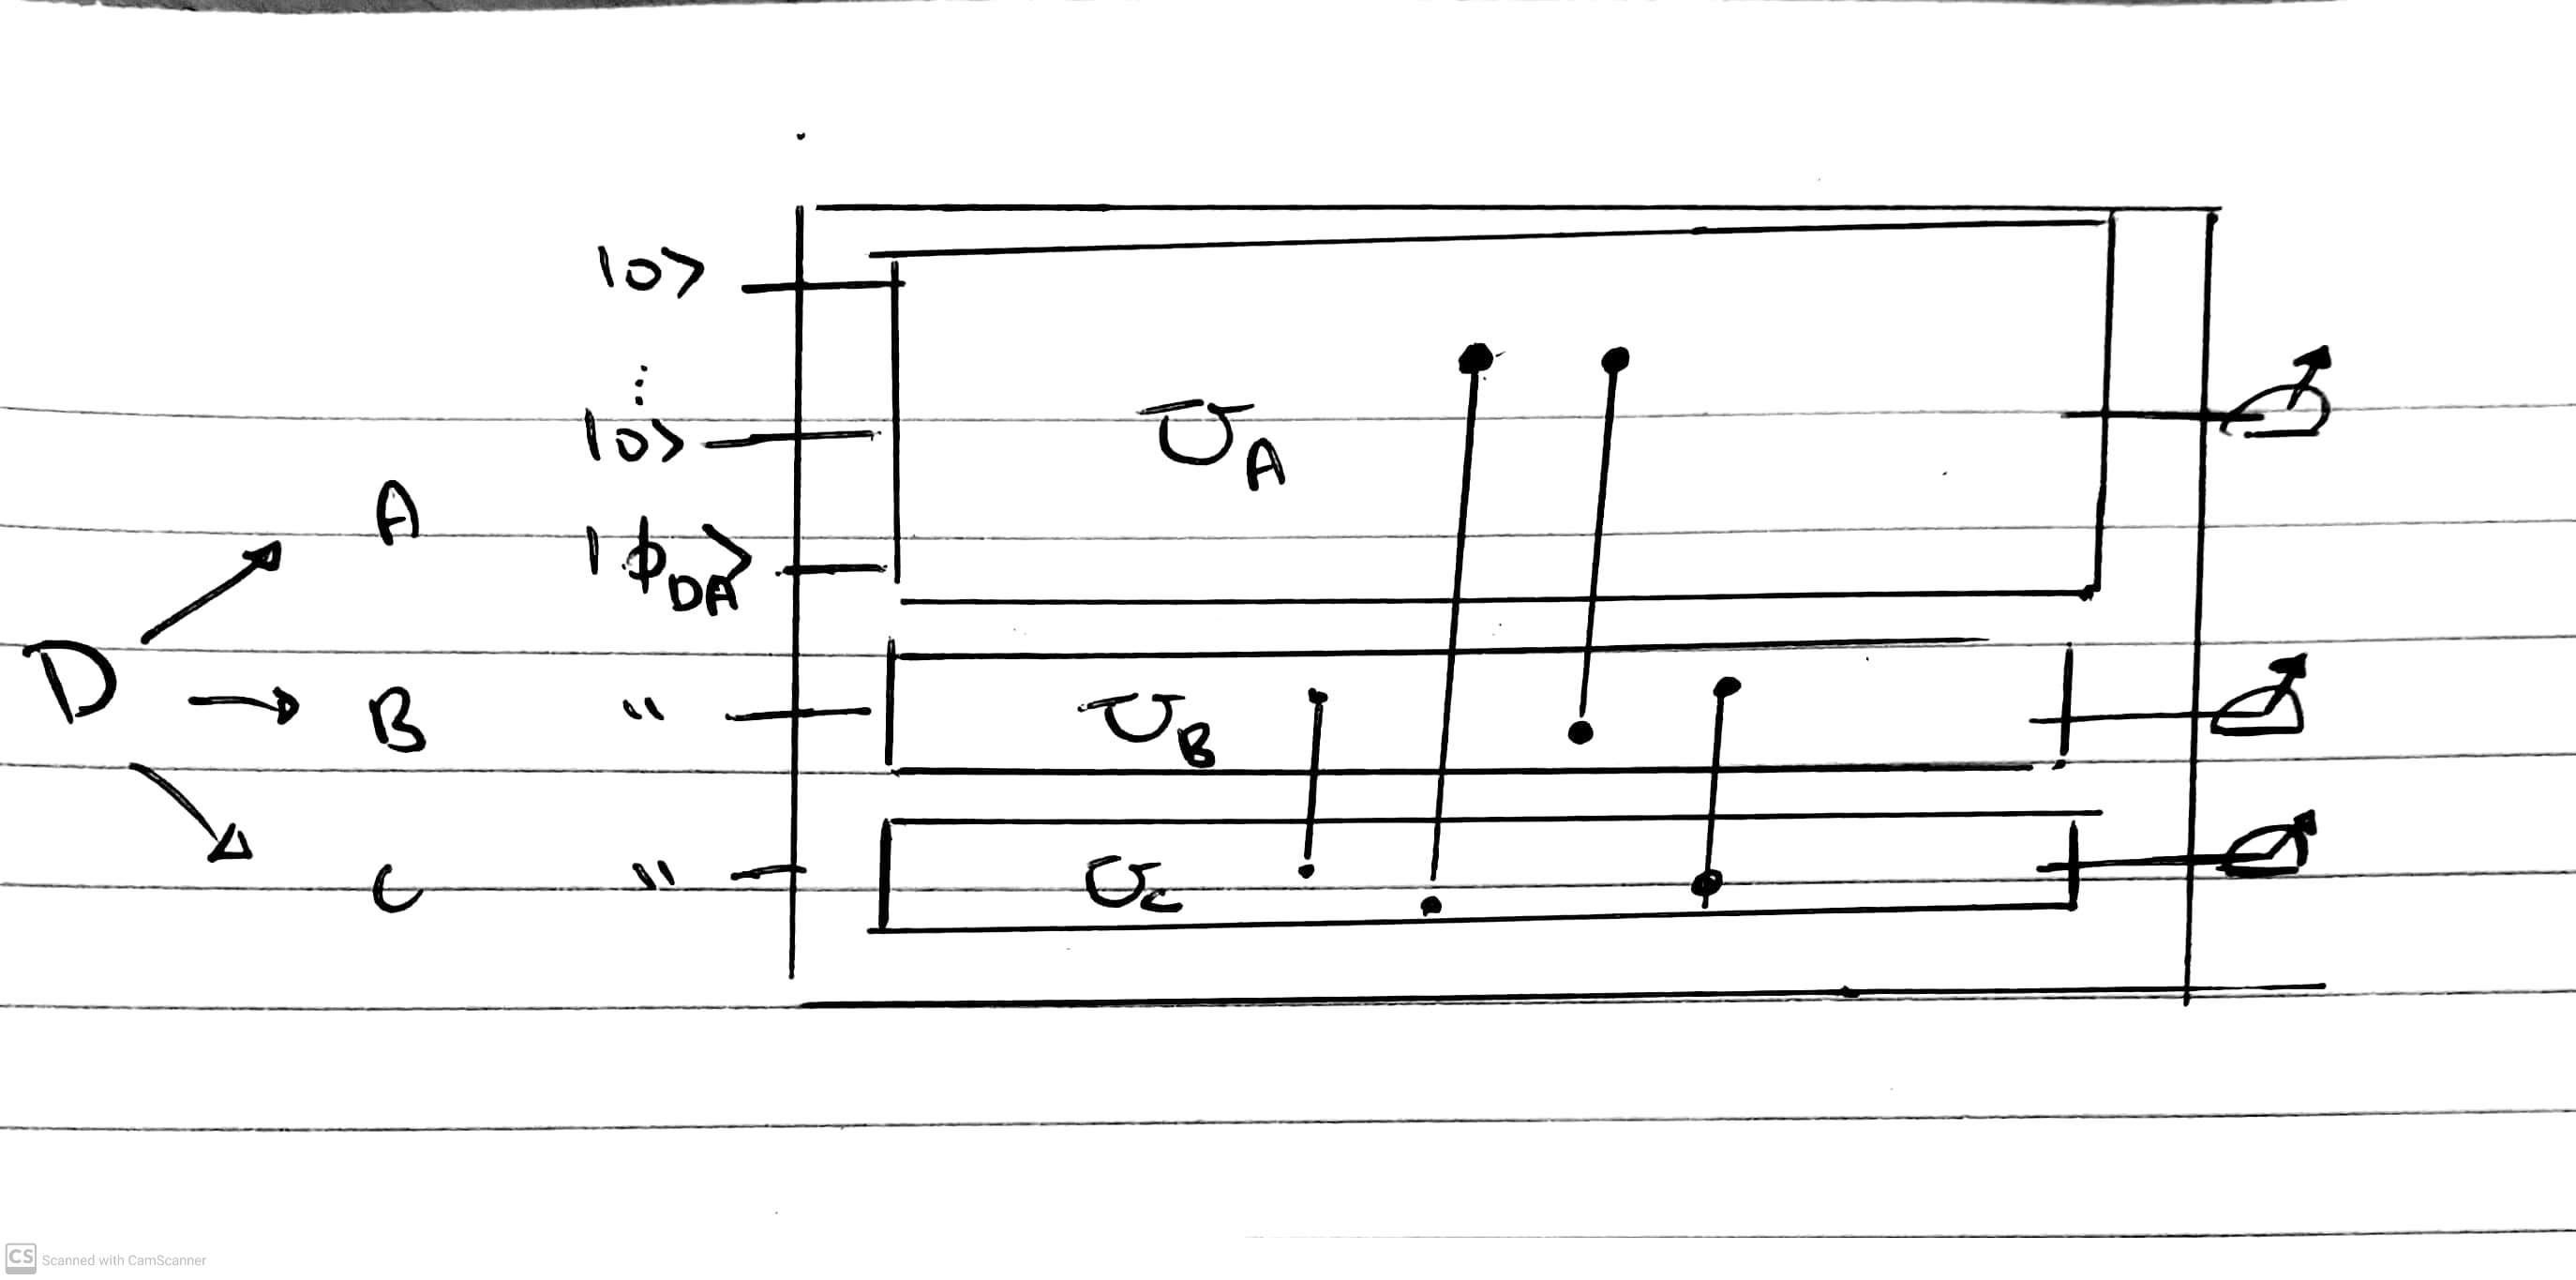
\includegraphics[scale=0.17]{images/avss protocol - Page 2.jpg}
\caption{ \(U_{\varepsilon}\) illustration. }
    \label{fig:simulation_cases}
\end{figure}

\begin{figure}[H]
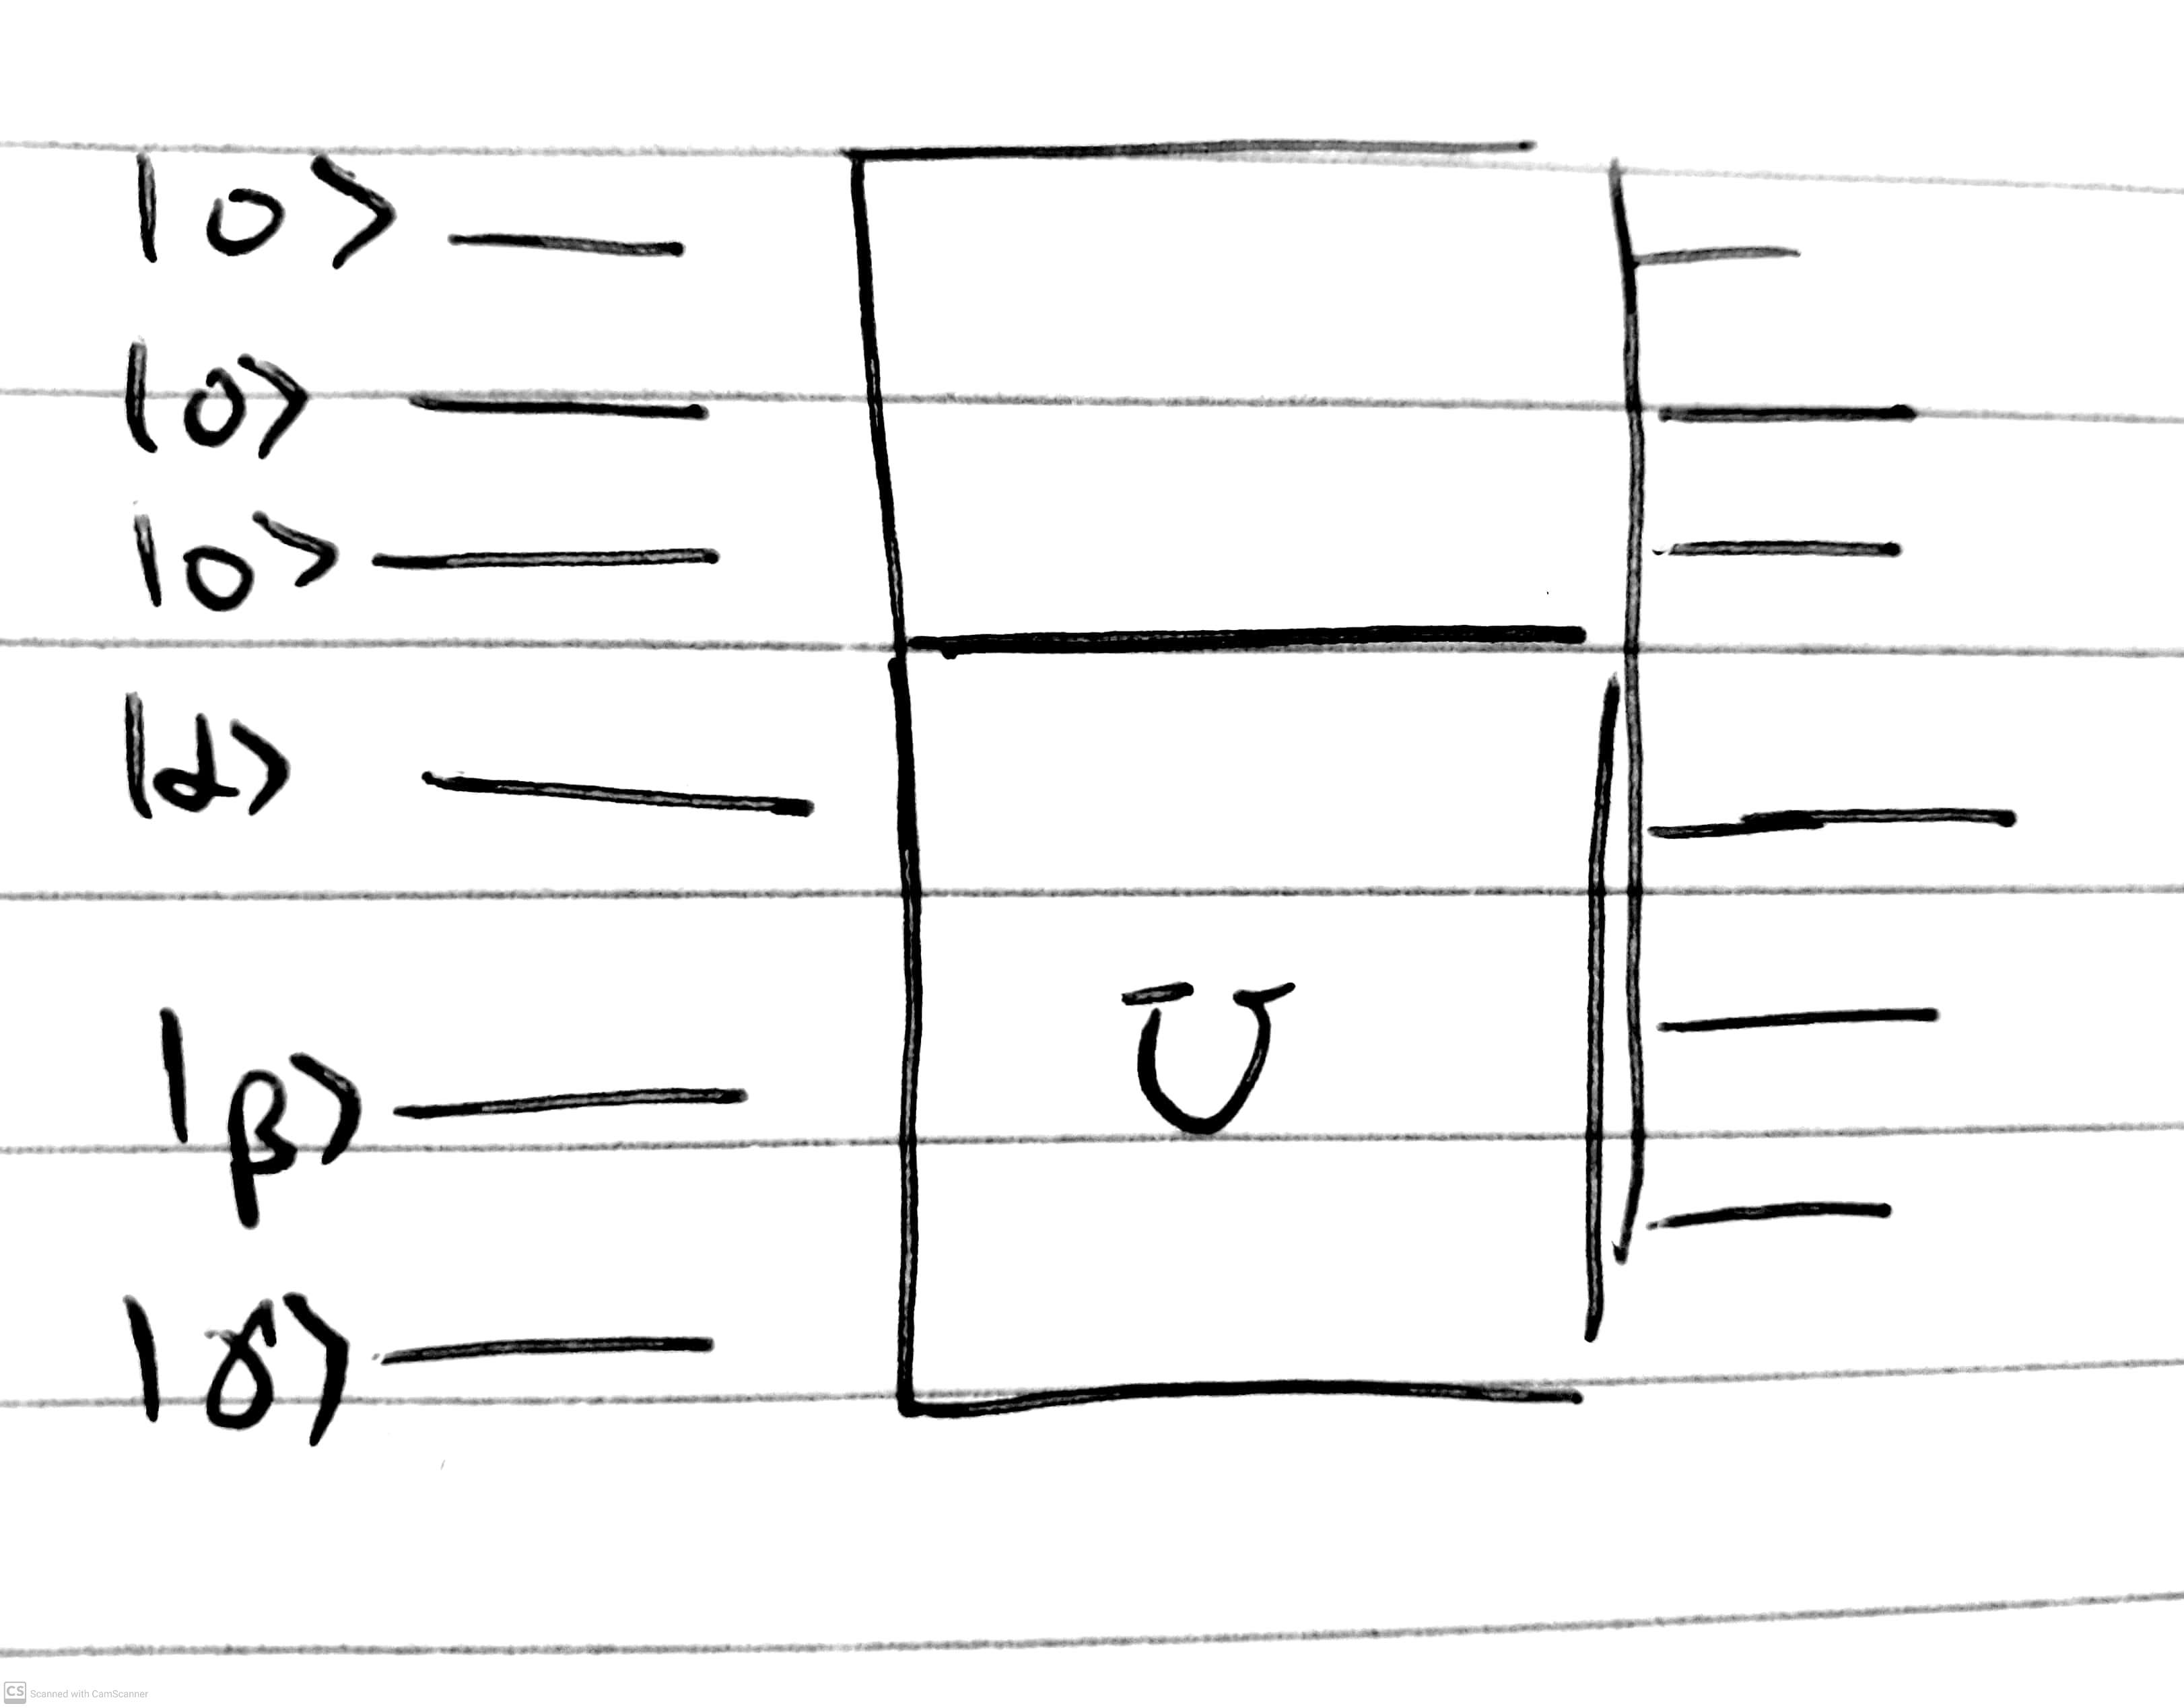
\includegraphics[scale=0.12]{images/avss protocol_3.jpg}
\caption{ \(U_{\varepsilon}\) illustration. }
    \label{fig:simulation_cases}
\end{figure}

\paragraph{Lemma II.} Consider the case when the dealer \(D\) is faulty. Then the resulting state of the computation over the input has nonzero weight for the an uncommitted ket.

\paragraph{Lemma III.} Consider the case when the party \(B\) is faulty. Then he could boost indistinguishability, which mean that he could amplify the weight of uncommitted ket.


\end{document}